\documentclass[11pt]{amsart}
\usepackage{amsmath, amssymb, amsthm}
\usepackage{todonotes}
\usepackage{cleveref}
\usepackage{tikz}
\usepackage{blkarray}
\usetikzlibrary{backgrounds,arrows,automata,positioning,shapes,shapes.geometric}


\DeclareMathOperator*{\argmax}{argmax}
\DeclareMathOperator*{\argmin}{argmin}

\theoremstyle{definition}
\newtheorem{theorem}{Theorem}[section]
\newtheorem{definition}[theorem]{Definition}
\newtheorem{conjecture}[theorem]{Conjecture}
\newtheorem{proposition}[theorem]{Proposition}
\newtheorem{corollary}[theorem]{Corollary}
\newtheorem{lemma}[theorem]{Lemma}
\newtheorem{claim}[theorem]{Claim}
\theoremstyle{remark}
\newtheorem*{remark}{Remark}
\newtheorem*{example}{Example}

\newenvironment{subproof}[1][\proofname]{%
  \renewcommand{\qedsymbol}{$\blacksquare$}%
  \begin{proof}[#1]%
}{%
  \end{proof}%
}


\title{Cooperation Is Provably Required in a Version of the Noisy Iterated Prisoner's Dilemma}
\author{Arvid Lunnemark. \\ \\
Supervised by: Michael Sipser}

\begin{document}
\tikzset{elliptic state/.style={draw,ellipse, text centered, text width=10em}}
\tikzstyle{block} = [rectangle, draw, fill=blue!20, 
    text width=5em, text centered, rounded corners, minimum height=4em]

\maketitle

\section{Introduction}

The prisoner's dilemma is a classic symmetric two-player game, where both players acting in their own best interests leads to an outcome that is not optimal for either of them. There are two actions, cooperate ($C$) and defect ($D$), with the payoffs represented by the matrix
\begin{equation*}
  \begin{matrix}
      &  C & D \\ 
    C &  (R, R) & (S, T) \\
    D & (T, S) & (P, P)
  \end{matrix}
  % \begin{blockarray}{cccccc}
  %   a & b & c & d & e \\
  %   \begin{block}{c(ccccc)}
  %     1 & 1 & 1 & 1 & 1 & f \\
  %     0 & 1 & 0 & 0 & 1 & g \\
  %     0 & 0 & 1 & 0 & 1 & h \\
  %     0 & 0 & 0 & 1 & 1 & i \\
  %     0 & 0 & 0 & 0 & 1 & j \\
  %   \end{block}
  %   \end{blockarray}
\end{equation*} \todo{copy the table from axelrod's book because it's much better and much clearer!!!}
where $T > R > P > S$ (the row player gets the first in each pair of numbers). Given the other player's action, a player always maximizes their payoff by choosing $D$, but with both doing so, the players end up in the $(D, D)$ state, which is worse for both than the $(C, C)$ state since $R > P$. The game can been used to model many real-world situations, including countries failing to act to stop climate change, doping in sport, and economic competition.

To make the game more interesting, one can consider playing it multiple times in a row with multiple players. One might loosely connect the repeated multiplayer game to evolution: why have humans evolved to cooperate with each other? In a seminal paper in 1980, Axelrod presented evidence that in a repeated setting with multiple players facing off in a tournament, cooperation can arise as the strategy of choice even for a selfish player \cite{axelrod1980effective}. In particular, the mostly cooperating Tit-for-tat strategy, depicted in \cref{tftfigure}, won his tournament. The idea is that even though Tit-for-tat loses when played against defecting strategies, that is outweighed by it being heavily rewarded when cooperating with other cooperating strategies.

\begin{figure}
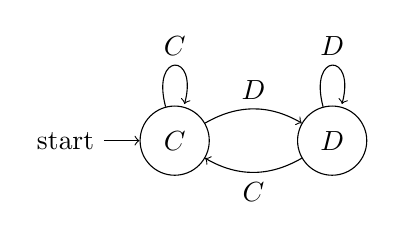
\begin{tikzpicture}[node distance=2cm]
  \node[state,initial] (s_0) {$C$};
  \node[state] (s_1) [right of=s_0] {$D$};

  \path[->] (s_0) edge [loop above] node {$C$} ();
  \path[->] (s_0) edge [bend left] node [above] {$D$} (s_1);
  \path[->] (s_1) edge [loop above] node {$D$} ();
  \path[->] (s_1) edge [bend left] node [below] {$C$} (s_0);
\end{tikzpicture}
  \centering
  \caption{The Tit-for-tat strategy. At any one point, it is in one of two states, taking the action corresponding to the label of the state. Upon perceiving its opponent's move, it decides to switch state if the opponent does something different.}
  \label{tftfigure}
\end{figure}

Clearly, however, the winning strategy in a tournament depends on the composition of strategies in that tournament. If all strategies had been of the type to always defect, Tit-for-tat would not have won the Axelrod tournament. Therefore, follow-up tournaments and simulations have been run, and perhaps surprisingly, most provide further evidence that cooperation is the prevailing strategy, as Axelrod summarizes in a 1981 book \cite{axelrod1981evolution}. There, he also introduces an evolutionary model that can be used for analyzing the game theoretically: strategies are considered to exist in a population that evolves over time in an evolutionary way (more successful strategies reproduce, and mutations can happen). In that context, a strategy is said to be evolutionarily stable if, supposing it controls a large share of the population, it resists being overtaken by any other strategy entering the population in small numbers. That is, populations of evolutionarily stable strategies form the equilibruim states of the evolutionary process, and thus, one may say that evolutionarily stable strategies are the ``best'' strategies.

In light of Axelrod's tournaments highlighting the effectiveness of cooperation, it has long been a goal to prove that a cooperating strategy like Tit-for-tat is evolutionarily stable. A few variants of this has been shown: First, Nowak has shown that in the finitely repeated game, a strategy that always defects is sometimes not evolutionarily stable \cite{nowak2004emergence}. Second, Binmore has shown that in the infinitely repeated game where strategies are modeled as finite automatons where having more states comes at a cost, a strategy needs to cooperate with itself to be stable \cite{binmore1992evolutionary}. And third, Fundenberg and Maskin have shown that a strategy needs to cooperate with itself to be stable also in the infinitely repeated game in the presence of a certain notion of infinitesimally small noise \cite{fundenberg1990evolution}.

Notably, all these results impose additional restrictions on the setup, and as noted by Fundenberg and Maskin, one has to do that: in the deterministic infinitely repeated game, one could create a strategy that can self-identify — if the opponent ever deviates from the pattern, the strategy resorts to defecting for the rest of the game. This strategy will be evolutionarily stable, but is not cooperative. 

In this paper, we, like Fundenberg and Maskin, choose the addition of noise as our restriction. In contrast to them, however, we present a model where, at every step, each strategy has a tiny probability $p$ of doing the wrong thing, which is arguably the most natural way of modeling noise. In \cref{sectionsetup}, we define the setup of our version of the problem in detail. Then, in \cref{sectionresults}, we state the two main results: that a strategy needs to be cooperative to be evolutionarily stable, and that such evolutionarily stable strategies exist. In \cref{sectionproofs}, we prove our results. Finally, in \cref{sectiondiscussion} we briefly discuss other potential ways of modeling the problem.

\section{Setup}
\label{sectionsetup}

In this section we define our setup. In summary, we consider the infinitely repeated prisoner's dilemma played by finite automata in infinite populations, evolving evolutionarily in the presence of noise.

\subsection{Formal Definition}

First, we define the reward function.

\begin{definition}
  The \textit{prisoner's dilemma} is a symmetric two-player game with two actions, cooperate ($C$) and defect ($D$), where, if player 1 selects action $a$ and player 2 selects action $b$, player 1 gets the reward
  \begin{equation*}
    r(a,b) = \begin{cases}
      R &\text{if $a = C, b = C$} \\
      T &\text{if $a = D, b = C$} \\
      S &\text{if $a = C, b = D$} \\
      P &\text{if $a = D, b = D$}
    \end{cases}
  \end{equation*}
  We require $T > R > P > S$ and $2R > T + S$.
\end{definition}

When we study the \textit{iterated} prisoner's dilemma, we want to look at strategies that determine their next move based on the history of previous moves. We restrict ourselves to strategies that can be implemented on a computer with finite memory.

\begin{definition}
  A \textit{strategy} $s$ is a Moore machine (finite automaton with outputs) over the input and output alphabet $\{C, D\}$. 
\end{definition}

We will consider strategies in the presence of noise. To model that, we will assume that a strategy has a probability $1-p$ of following the correct transition and a probability $p$ of following the incorrect transition, at every step. Note that this models noise in \textit{perception}. One could also imagine modeling noise in \textit{action taken}, but it is easy to see that the two are equivalent up to a change in the values of $R, T, S$ and $P$.

We can now begin to define the outcome of two strategies playing against each other in the infinitely repeated game. We do this using Markov chains.

\begin{definition}
  Suppose that strategy $s_1$ plays against strategy $s_2$. This defines an \textit{$s_1$-$s_2$ Markov chain} where each state is a tuple $(c_1,c_2)$ with $c_1$ being a state in $s_1$ and $c_2$ a state in $s_2$. The transition probabilities are defined in the obvious way:
  \begin{equation*}
    p_{(c_1,c_2) \to (c_1', c_2')} = p_{c_1 \to c_1'} \cdot p_{c_2 \to c_2'},
  \end{equation*}
  where $p_{c_1 \to c_1'}$ is $1-p$ if the output of $s_2$ at state $c_2$ causes $c_1$ to transition to $c_1'$, and is $p$ if the opposite of that output causes that transition; $p_{c_2 \to c_2'}$ is defined similarly.
\end{definition}

Markov chains naturally leads themselves to the study of limiting cases.

\begin{definition}
  \label{timeaveragedistribution}
  The \textit{time average distribution} of the $s_1$-$s_2$ Markov chain given the start state $(a, b)$, denoted $\pi^{(a, b)}$, is the distribution such that \begin{equation*}
    \pi_{c_1, c_2}^{(a, b)} = E \left[ \text{fraction of time in state $(c_1,c_2)$} \mid \text{initial state is } (a, b)  \right]
  \end{equation*}
  where the expected fraction of time is taken over the infinite sequence $(X_0, X_1, \ldots)$.
\end{definition}

We will often use $\pi$ to refer to $\pi^{(a_0, b_0)}$ where $a_0$ is the initial state of $s_1$ and $b_0$ is the initial state of $s_2$.

\begin{definition}
  \label{payofftimeaverage}
  Let $r(c_1, c_2)$ refer to the reward that $s_1$ gets when $s_1$ takes the action in state $c_1$ and $s_2$ takes the action in state $c_2$. Then, the \textit{payoff that $s_1$ gets when playing against $s_2$} is
  \begin{equation*}
    v_{s_1}(s_2) = \sum_{(c_1,c_2)} \pi_{c_1,c_2} \cdot r(c_1, c_2),
  \end{equation*}
  where the sum is taken over all states $(c_1,c_2)$ in the $s_1$-$s_2$ Markov chain.
\end{definition}

For notational convenience, we may also make $r(c_1, c_2)$ into a vector, denoted by $r$, and write this as the dot product \begin{equation*}
  v_{s_1}(s_2) = \pi \cdot r.
\end{equation*}

That is, the payoff that $s_1$ gets when playing against $s_2$ is simply an average of the reward it gets in each possible state of the Markov chain weighted by the fraction of time that is spent there.

\iffalse
We use the notation $G_{s_1,s_2}(c_1,c_2)$ to refer to the vector $(G_{s_1}(c_1), G_{s_2}(c_2))$, and we use $S_{s_1,s_2}$ to refer to the set of all states in the Markov chain.

\begin{definition}
  \label{strategypayoffs}
  Let $X_t$ be the random variable designating which state the $s_1$-$s_2$ Markov chain is in at time $t$. The \text{payoff} of strategy $s_1$ when played against strategy $s_2$ is 
  \begin{equation*}
    v_{s_1}(s_2) = E \left[ \lim_{T \to \infty} \frac{1}{T} \sum_{t=0}^T r(G_{s_1,s_2} (X_t)) \Bigm| X_0 = (c_{\text{start}}(s_1), c_{\text{start}}(s_2)) \right]
  \end{equation*}
\end{definition}

That is, when $s_1$ plays against $s_2$, we define its payoff to be the average payoff over all possible infinite sequences of moves. Note that the expectation is taken over the infinite sequence $(X_0, X_1, \ldots)$. The limit inside is thus simply a normal time average limit of bounded real numbers, which clearly exists. 

We will now introduce the notion of a time average distribution which will lead us to a second way of defining the payoff $v_{s_1}(s_2)$. \todo{is this really necessary?? should i pick one or the other?? should i move one of them to the next section? which one is easier to understand? do they trivially say the same thing?}

\begin{definition}
  \label{timeaveragedistribution}
  The \textit{time average distribution} of the $s_1$-$s_2$ Markov chain given the start state $(a, b)$, denoted $\pi^{(a, b)}$, is the distribution such that \begin{equation*}
    \pi_{c_1, c_2}^{(a, b)} = E \left[ \text{fraction of time in state $(c_1,c_2)$} \mid \text{initial state is } (a, b)  \right]
  \end{equation*}
  where the expected fraction of time is taken over the infinite sequence $(X_0, X_1, \ldots)$.
\end{definition}

We will use $\pi$ to refer to $\pi^{(c_{\text{start}}(s_1), c_\text{start}(s_2))}$.

\begin{lemma}
  \label{payofftimeaverage}
  The payoff when $s_1$ plays against $s_2$ is
  \begin{equation*}
    v_{s_1}(s_2) = \sum_{(c_1,c_2) \in S_{s_1,s_2}} \pi_{c_1,c_2} \cdot r(G_{s_1}(c_1),G_{s_2}(c_2)).
  \end{equation*}
\end{lemma}

We may also make $r(G_{s_1}(c_1),G_{s_2}(c_2))$ into a vector, denoted by $r$, and write this as the dot product \begin{equation*}
  v_{s_1}(s_2) = \pi \cdot r.
\end{equation*}

\todo{I think the best way to handle this is to remove the expected value definition altogether. just do the time average distribution and skip the proof of the lemma. it is honestly a very natural definition}

\begin{proof}[Proof of \cref{payofftimeaverage}]
  The key idea is that a time average sum where each element is one of finitely many values can be written as a frequency-weighted finite sum instead. Let $I_{c_1,c_2,t}$ be the indicator variable that is 1 if $G_{s_1,s_2}(X_t) = (c_1,c_2)$ and 0 otherwise.  Then, we can write \begin{equation*}
    \lim_{T \to \infty} \frac{1}{T} \sum_{t = 0}^T r(G_{s_1,s_2}(X_t)) = 
    \lim_{T \to \infty}\frac{1}{T} \sum_{t = 0}^T \sum_{(c_1,c_2) \in S_{s_1,s_2}} r(c_1,c_2) \cdot I_{c_1,c_2,t}
  \end{equation*}
  We may now exchange the order of summation and move the finite sum out of the limit, to get \begin{equation*}
    \lim_{T \to \infty}\frac{1}{T} \sum_{t = 0}^T \sum_{(c_1,c_2) \in S_{s_1,s_2}} r(c_1,c_2) \cdot I_{c_1,c_2,t}
    = \sum_{(c_1,c_2) \in S_{s_1,s_2}} r(c_1,c_2) \cdot \lim_{T \to \infty} \sum_{t=0}^T \frac{I_{c_1,c_2,t} }{T}
  \end{equation*}
  We can now use \cref{strategypayoffs} and linearity of expectation to find that
  \begin{equation*}
    v_{s_1}(s_2) = \sum_{(c_1,c_2) \in S_{s_1,s_2}} r(c_1, c_2) E \left[ \lim_{T \to \infty} \sum_{t=0}^T \frac{I_{c_1,c_2,t}}{T} \bigm| X_0 = (c_{\text{start}}(s_1), c_{\text{start}}(s_2))
    \right]
  \end{equation*}
  Finally, we note that this is exactly the statement of \cref{payofftimeaverage}, which proves our lemma.
\end{proof}

Appendix A contains more details on time average distributions. In particular, if a unique stationary distribution exists, it is equal to the time-average distribution, which enables us to quickly find the time-average distribution in many cases.

\fi

We're now ready to look at how strategies interact.

\begin{definition}
  A \textit{population} of strategies $P = (S, f)$ is a set $S$ of strategies and a function $f : S \to (0,1]$ such that $\sum_{s \in S} f(s) = 1$, representing the frequency of each strategy in the population.
\end{definition}

\begin{definition}
  The \textit{fitness} of a strategy $s$ in a population $P = (S, f)$ is \begin{equation*}
    F(s) = \sum_{s' \in S} f(s') v_s(s').
  \end{equation*}
\end{definition}

One can think of this as saying that we have infinitely many members of the population, interacting with each other evenly, and that the fitness of a strategy is its expected payoff. Having infinitely many interactions like this justifies the usage of expectation when definining $v_{s_1}(s_2)$.

We can now use the fitness of a strategy to compare it with other strategies in the same population. If a strategy $s_1$ has a higher fitness than another strategy $s_2$, we say that the frequency of $s_1$ will increase at the expense of the frequency of $s_2$, in the next step of the evolutionary process. This is getting us close to how we want to define stable strategies; our next move is looking not only at a single evolutionary step, but the entire evolutionary process.

\begin{definition}
  A strategy $s_1$ is \textit{$\epsilon$-invadable} if there exists a strategy $s_2$ such that in all populations $P$ with $S = \{s_1,s_2\}$ and $f(s_2) \geq \epsilon$, we have 
  \begin{equation*}
    \label{fitnesscond}
    F(s_2) > F(s_1)
  \end{equation*}
\end{definition}

That is, if $s_1$ is $\epsilon$-invadable, there exists a strategy $s_2$ that can start as only a tiny fraction $\epsilon$ of the total population, and consistently have higher fitness than $s_1$, eventually causing $s_2$ to overtake and then eliminate $s_1$ completely. We are now finally ready to define evolutionary stability.

\begin{definition}
  A strategy $s_1$ is \textit{evolutionarily stable} if there exists parameters $p_0$ and $\epsilon_0$ with $0 < p_0, \epsilon_0 < 1$, such that for all $p < p_0$, and all $\epsilon < \epsilon_0$, $s_1$ is not $\epsilon$-invadable.
\end{definition}

\todo{separate this definition out into a pure evolutionarily stable definition, and then an evolutionarily stable for infinitesimally small probabilities definition?? would make interpretation much clearer.}

That is, a strategy $s_1$ is evolutionarily stable if, as the noise probability $p$ goes to 0, it can withstand invasion attempts from any strategy that starts off as a tiny fraction of the population.

\subsection{Interpretation}

Having concluded our formal definition of evolutionary stability, it might be helpful to see examples of concrete setups in which this definition makes sense.

Consider the following world. 

\todo{WRITE THIS SECTION?? I'M NOT SURE THAT MY MODEL MAKES MUCH SENSE ANYMORE THOUGH, BECAUSE IT REQUIRES PEOPLE TO PLAY AGAINST THEMSELVES WHICH IS A NONO. also the probability going to 0 does not really make sense}


\section{Results}
\label{sectionresults}

We can now state our results! Together, the following theorem and conjecture imply that in the setup described here, mutual cooperation arises as the only stable choice.

\begin{theorem}
  \label{evolutionarystable1}
  Suppose that a strategy $s_1$ is evolutionarily stable. Then $\lim_{p \to 0} v_{s_1}(s_1) = R$.
\end{theorem}

\begin{conjecture}
  \label{pavlovtheorem}
  Suppose that $2R > T + P$. Then, the Pavlov strategy, depicted in \cref{pavlovfigure}, is evolutionarily stable.
\end{conjecture}

\begin{figure}
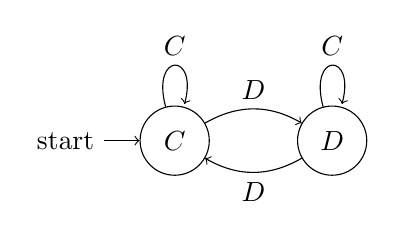
\begin{tikzpicture}[node distance=2cm]
  \node[state,initial] (s_0) {$C$};
  \node[state] (s_1) [right of=s_0] {$D$};

  \path[->] (s_0) edge [loop above] node {$C$} ();
  \path[->] (s_0) edge [bend left] node [above] {$D$} (s_1);
  \path[->] (s_1) edge [loop above] node {$C$} ();
  \path[->] (s_1) edge [bend left] node [below] {$D$} (s_0);
\end{tikzpicture}
  \centering
  \caption{The Pavlov strategy. Similar to but not the same as the Tit-for-tat strategy.}
  \label{pavlovfigure}
\end{figure}


\begin{remark}
  Tit-for-tat, depicted in \cref{tftfigure}, is not evolutionarily stable. 
  When played against itself, it ends up spending just as much time in the defection state as in the cooperation state, because as soon as one mistake is made, it goes into a mutual defection cycle with its clone that is only broken by an additional mistake.
  Thus, $v_s(s)$ where $s$ is Tit-for-tat is much smaller than $R$, which means that it is not evolutionarily stable by \cref{evolutionarystable1}.
\end{remark}


\section{Proofs}
\label{sectionproofs}

In this section, we prove our results from the previous section.

\subsection{The time average distribution}

Before we prove \cref{evolutionarystable1}, we need to understand what the payoff $v_{s_1}(s_2)$ really means. In this subsection, we prove a series of lemmas that characterize the time average distribution, and consequently $v_{s_1}(s_2)$.

\begin{lemma}
  \label{timeaverageisstationary}
  The time average distribution $\pi^{(a,b)}$, for any starting state $(a,b)$, is a stationary distribution of the Markov chain. That is, if $M$ is the transition matrix of the Markov chain, we have $M \pi^{(a,b)} = \pi^{(a,b)}$.
\end{lemma}

We state this lemma without proof, as it is a fairly standard result. Important to note is that the time average distribution is not necessarily a \textit{unique} stationary distribution, as we make no assumptions that our Markov chain be ergodic.

\begin{definition}
  A \textit{strongly connected component} of a directed graph is a subgraph where there is a path from every node to every other node.
\end{definition}

\begin{definition}
  An \textit{absorbing component} of a directed graph is a subgraph where there are no edges from vertices inside the component to vertices outside it.
\end{definition}

We may also put both of the terms together and talk about absorbing strongly connected components, which, as shown by the next few lemmas, are useful.

\begin{lemma}
  \label{lemmaabsorbinghasuniquetimeaverage}
  An absorbing strongly connected component has a unique time average distribution, i.e., the time average distribution does not depend on the start state.
\end{lemma}

\begin{proof}
  It is well known that a strongly connected (also known as irreducible) Markov chain has a unique stationary distribution. Since the time average distribution is stationary by \cref{timeaverageisstationary}, it thus also has to be unique.
\end{proof}

\begin{lemma}
  \label{timeaveragedistributiondecomposition}
  Let $\mathcal{A}$ be the set of absorbing strongly connected components of the $s_1$-$s_2$ Markov chain. For every $S \in \mathcal{A}$, let $\pi^{(S)}$ be its unique time average distribution. Then, for some probabilities $p_{S}$ with $\sum_{S \in \mathcal{A}} p_{S} = 1$, corresponding to the time average probabilities of ending up in the absorbing strongly connected component $S$, we have \begin{equation*}
    \pi = \sum_{S \in \mathcal{A}} p_{S} \cdot \pi^{(S)}.
  \end{equation*}
\end{lemma}

Finally, we can characterize the absorbing strongly connected components of the $s_1$-$s_2$ Markov chain in terms of the absorbing SCCs of $s_1$ and $s_2$ separately.

\begin{lemma}
  \label{absorbingstronglyconnectedcomponentscartesianproduct}
  Let $\mathcal{A}_1$ be the set of absorbing strongly connected components of $s_1$, and similarly, let $\mathcal{A}_2$ be the set of absorbing strongly connected components of $s_2$. If $\mathcal{A}$ is the set of absorbing strongly connected components of the $s_1$-$s_2$ Markov chain, then 
  \begin{equation*}
    \mathcal{A} = \{H \times K \mid H \in \mathcal{A}_1 \text{ and } K \in \mathcal{A}_2\},
  \end{equation*}
  where $A \times B$ is the cartesian product $A \times B = \{(a, b) \mid a \in A \text{ and } b \in B\}$.
\end{lemma}

Now that we know more about the time average distribution, we are also interested in proving that the payoff function behaves nicely.

\begin{lemma}
  \label{limitvexists}
  The limit \begin{equation*}
    \lim_{p \to 0} v_{s_1}(s_2)
  \end{equation*}
  exists, for any strategies $s_1$ and $s_2$.
\end{lemma}
\begin{proof}
  By definition, \begin{equation*}
    v_{s_1}(s_2) = \pi \cdot r.
  \end{equation*}

  By \cref{timeaverageisstationary}, $\pi$ is a stationary distribution. In particular, if $M$ is the transition matrix for the $s_1$-$s_2$ Markov chain, then $\pi$ is an eigenvector of $M$ with eigenvalue 1. This implies that $\pi$ is in the nullspace of $M - I$. Thus, we can find $\pi$ by solving for $X$ in $(M - I)X = 0$. If we solve this using Gaussian elimination and back substitution, it is clear that the entries of $\pi$ will be on the form $\frac{f(p)}{g(p)}$ where $f$ and $g$ are polynomials in $p$, since each 
  entry of $M$ is a second-degree polynomial in $p$. This is continuous for all $p$ where $g(p) \neq 0$, and since $g$ will have a finite degree it is therefore continuous in a small right neighborhood of 0. Finally, note that $v_{s_1}(s_2)$ is between $S$ and $T$, which in conclusion means that the limit of it as $p$ goes to 0 tends to a finite number, as desired.
\end{proof}

\begin{lemma}
  \label{neverbetterthanr}
  For any strategy $s$,
  \begin{equation*}
    v_{s}(s) \leq R
  \end{equation*}
\end{lemma}
\begin{proof}
  For notational simplicity, we will let $s_1$ and $s_2$ be two copies of strategy $s$. Then, $v_{s}(s) = v_{s_1}(s_2) = v_{s_2}(s_1)$. By definition, we have
  \begin{equation*}
    v_{s_1}(s_2) = \sum \pi_{c_1,c_2} \cdot r(c_1, c_2)
  \end{equation*}
  and
  \begin{equation*}
    v_{s_2}(s_1) = \sum \pi_{c_2,c_1} \cdot r(c_2, c_1).
  \end{equation*}
  Note that $\pi_{c_1,c_2}$ and $\pi_{c_2,c_1}$ refer to the same state, so we thus have \begin{equation*}
    v_{s_1}(s_2) + v_{s_2}(s_1) = \sum \pi_{c_1,c_2} \cdot (r(c_1,c_2) + r(c_2,c_1))
  \end{equation*}
  which implies that \begin{equation*}
    v_s(s) = \sum \left( \pi_{c_1,c_2} \cdot \frac{r(c_1,c_2) + r(c_2,c_1)}{2} \right).
  \end{equation*}
  Now, note that $r(c_1,c_2) + r(c_2,c_1) \in \{R + R, S + T, T+S, P + P\}$. Since $P < R$ and $T + S < 2R$, we thus find that \begin{equation*}
    v_s(s) \leq \sum \pi_{c_1,c_2} \cdot R = R \sum \pi_{c_1,c_2} = R,
  \end{equation*}
  as desired.
\end{proof}

\subsection{Evolutionary Stability Requires Cooperation}

  We are now finally ready to prove that to be evolutionarily stable, a strategy needs to cooperate with a clone of itself.

    \begin{proof}[Proof of \cref{evolutionarystable1}]
      Suppose that the strategy $s_1$ is such that it is \textit{not} true that \begin{equation*}
        \lim_{p \to 0 } v_{s_1}(s_1) = R.
      \end{equation*}
      By \cref{limitvexists} and \cref{neverbetterthanr}, this assumption implies that the limit is strictly less than $R$. Define $\gamma = \lim_{p \to 0} v_{s_1}(s_1)$. Then,
      \begin{equation*}
        \gamma < R.
      \end{equation*}
      
      We want to prove that $s_1$ is not evolutionarily stable. 
      
      To do that, we want to prove that for all $p_0, \epsilon_0 \in (0,1)$, there exists $p < p_0$ and $\epsilon < \epsilon_0$, such that $s_1$ is $\epsilon$-invadable. We choose $\epsilon = \epsilon_0 / 2$, and present a strategy $s_2$ that can invade $s_1$ for all $p$ that are sufficiently small.


      The underlying idea is to construct $s_2$ such that $s_1$ can see no difference between itself and $s_2$, while $s_2$, on the other hand, can. If we succeed in doing so, we will have that $v_{s_1}(s_2) = v_{s_2}(s_1) = v_{s_1}(s_1)$, and can construct $s_2$ such that it always cooperates when it recognizes itself, thereby yielding $v_{s_2}(s_2) = R$. This would give $s_2$ a higher fitness than $s_1$. The rest of this proof executes this plan in detail.

      We create the strategy $s_2$ as follows. First, we copy all of $s_1$ into $s_2$. Let $\mathcal{A}_1$ be the set of
       absorbing strongly connected components of $s_1$. The key idea, now, is to replace each original absorbing strongly connected component $H \in \mathcal{A}_1$ with a new absorbing component $K_H$, which has the capability of identifying itself.

      We now construct a $K_H$ for each $H$. \Cref{c2flowchart} shows the high-level construction of $K_H$.
       All of the steps succeed with probability $1 - O(p)$. The first step makes sure that $K_H$ does not deviate from $s_1$ at all
        until $s_1$ has reached an absorbing strongly connected component. 
       Once $s_1$ is in an absorbing strongly connected component, \cref{lemmaabsorbinghasuniquetimeaverage} tells us that the time average distribution does not depend on the particular start state in that component, which means that even if $s_1$ after this point ``figures out'' that it is not playing against itself anymore, there is nothing it can do about it (since it also cannot escape the component). 
      The second step in the construction of $K_H$ makes sure that if $s_2$ is playing against itself, it is in sync with its clone; that is, with probability $1 - O(p)$, both copies of $s_2$ will be in the exact same state after the second step. 
      The third step now figures out what action $s_1$ would take at some large finite time $T$. 
      Then, $K_H$ outputs the exact opposite action at time $T$. 
      At that point, if its opponent outputs $s_1$'s expected action, it transitions into the absorbing strongly connected component $H_\text{copy}$, which is just an exact copy of $H$, but if its opponent outputs the opposite of that action, it has successfully recognized itself and enters an always cooperating state.

      \begin{figure}
        \centering
        \begin{tikzpicture}[node distance=0.9cm,initial text=]
          \node[elliptic state, initial, initial where=above] (c_0) {1. Wait until $s_1$ is in an absorbing SCC, while simulating $H$.};
          \node[elliptic state] (c_1) [below=of c_0] {2. Sync $s_2$.};
          \node[elliptic state] (c_3) [below=of c_1] {3. Figure out what action that $s_1$ will take right after this.};
          \node[state] (c_4) [below left=of c_3] {$C$};
          \node[state] (c_5) [below right=of c_3] {$D$};
          \node[state] (c_6) [below=of c_5] {$C$};
          \node[elliptic state] (c_7) [below=of c_4] {$H_\text{copy}$ \\(an exact copy of $H$)};


          \path[->] (c_0) edge (c_1);
          \path[->] (c_1) edge (c_3);
          \path[->] (c_3) edge node [above left] {$s_1$ will take $D$} (c_4);
          \path[->] (c_3) edge node [above right] {$s_1$ will take $C$} (c_5);
          \path[->] (c_4) edge node [below, pos=0.1] {$C$} (c_6);
          \path[->] (c_5) edge node [right] {$D$} (c_6);
          \path[->] (c_4) edge node [left] {$D$} (c_7);
          \path[->] (c_5) edge node [below, pos=0.1] {$C$} (c_7);
          \path[->] (c_6) edge [loop right] (c_6);
          % \path[->] (c_0) edge node [above right] {$\bar{\alpha}$} (c_1);
          % \path[->] (c_1) edge [loop right] node [right] {$C,D$} ();
          % \path[->] (c_0) edge node [above left] {$\alpha$} (c_prime);
          % \path[->] (c) edge node [below left] {$\alpha$} (c_prime);
        \end{tikzpicture}
        \caption{High level construction of $K_H$, the absorbing component replacing $H$ when creating $s_2$ in the proof of \cref{evolutionarystable1}. Note that $K_H$ contains exactly 2 absorbing strongly connected components.}
        \label{c2flowchart}
      \end{figure}
      
      This concludes the high-level construction of $s_2$. We now want to prove that this $s_2$ can in fact invade $s_1$. To do that, we will first assume that the below 3 claims are correct, i.e., that the construction is possible and works as specified, and then finish the proof of our theorem using those assumptions. Once that's done, we will prove the 3 claims.

      \begin{claim}
        \label{claimcanwaitfors1}
        We can construct a non-absorbing component with behavior indistinguishable from the behavior of component $H$, such that when we leave the component, $s_1$ will be in an absorbing strongly connected component with probability $1 - O(p)$.
      \end{claim}

      \begin{claim}
        \label{claimcansyncs2}
        We can construct a non-absorbing component placed after the first component, such that if $s_2$ plays against itself, both clones transition out of the component at the exact same time with probability $1 - O(p)$.
      \end{claim}

      \begin{claim}
        \label{claimcanfigureout}
        We can construct a non-absorbing component with a finite number of maximum steps that, supposing that $s_2$ plays against $s_1$, can figure out what action $s_1$ will take at the exact timestep following the transition out of the component.
      \end{claim}

      We now finish our proof.

      \begin{claim}
        \label{claimpayoffs}
        Given the above construction of $s_2$, the payoffs are as follows.
      \begin{align*}
        v_{s_1}(s_1) &= \gamma + O(p) \\
        v_{s_1}(s_2) &= \gamma + O(p) \\
        v_{s_2}(s_1) &= \gamma + O(p) \\
        v_{s_2}(s_2) &= R + O(p)
      \end{align*}
      \end{claim}
      \begin{subproof}

        By our definition of $\gamma$, we have that $v_{s_1}(s_1) = \gamma + O(p)$.

        Consider now the case of $s_1$ playing against $s_2$. Suppose that $s_2$ ends up in the absorbing component $K_H$. By \cref{claimcanwaitfors1}, with probability $1 - O(p)$, $s_2$ is indistinguishable from $s_1$ until $s_1$ also reaches an absorbing strongly connected component, which we call $H'$. This means that the probability for reaching the absorbing component $(C_1', C_2)$ in the $s_1$-$s_2$ Markov chain, is up to a factor of $1 - O(p)$ the same as if we hadn't replaced $C_1$ by $C_2$, which is just the probability of reaching the absorbing component $(C_1', C_1)$ in the $s_1$-$s_1$ Markov chain. Thus, 
        \begin{multline*}
          P(\text{$s_1$-$s_2$ chain ends up in $(C_1', C_2)$}) \\ = (1 - O(p)) P(\text{$s_1$-$s_1$ chain ends up in $(C_1', C_1)$})
        \end{multline*}
        Now, by \cref{claimcanfigureout}, the probability that $s_2$ enters the absorbing strongly connected component $C_1$ after having gotten to $C_2$ is $1 - O(p)$, and that it enters the always cooperating component $C_c$ is $O(p)$. Thus,
        \begin{align*}
          P(\text{$s_1$-$s_2$ chain ends up in $(C_1',C_1)$}) &= P(\text{$s_1$-$s_1$ chain ends up in $(C_1',C_1)$}) + O(p) \\
          P(\text{$s_1$-$s_2$ chain ends up in $(C_1',C_c)$}) &= O(p)
        \end{align*}
        That is, when $s_1$ plays against $s_2$, the absorbing strongly connected components are mostly the same, with mostly the same probabilities. 
        Now, we can calculate $\tau$, the time average distribution of the $s_1$-$s_2$ Markov chain:

        \todo{this is nonsensical here!! i should really try to explain this better!!!!!}

        % By definition, $v_{s_1}(s_1) = \gamma$. By \cref{timeaveragedistributiondecomposition}, the time average distribution of the $s_1$-$s_1$ Markov chain $\pi$ is \begin{equation*}
        %   \pi = \sum_{(C_1, C_1') \in \mathcal{C}_1 \times \mathcal{C}_1} p_{(C_1, C_1')} \cdot \pi^{(C_1, C_1')}
        % \end{equation*}
        % When creating $s_2$, we replaced each $C_1$ by a $C_2$, containing two absorbing strongly connected components: a copy of $C_1$, which we call $C_{1, \text{copy}}$ and the always cooperating $C_c$. This means that the condensation of the $s_1$-$s_2$ Markov chain is the same as the condensation of the $s_1$-$s_1$ Markov chain, except that each absorbing strongly connected component has been replaced by two. That is, the absorbing strongly connected component $(C_1, C_1')$ of the $s_1$-$s_1$ chain has become both $(C_1, C_{1, \text{copy}})$ and $(C_1, C_c)$ in the $s_1$-$s_2$ chain. Then, we find by our construction, that 
        % \begin{align}
        %   \label{c1c1copy}
        %   p_{(C_1, C_{1, \text{copy}})} &= (1 - O(p)) p_{(C_1, C_1')} \\
        %   p_{(C_1, C_c)} &= O(p) p_{(C_1, C_1')}
        % \end{align}
        % This equation is true because when $s_2$ plays against $s_1$, it identifies the action $A$ that $s_1$ will take at time $A$ with probability $(1 - O(p))$, and upon seeing that transitions to $C_{1, \text{copy}}$ with probability $(1-p)$.

        \begin{align*}
          \tau &= \sum_{(C_1, C') \in \mathcal{C}_1 \times \mathcal{C}_2} p_{(C_1, C')} \cdot \pi^{(C_1, C')} \\
          &= \sum_{(C_1, C_{1, \text{copy}})} p_{(C_1, C_{1, \text{copy}})} \cdot \pi^{(C_1, C_{1, \text{copy}})} + \sum_{(C_1, C_c)} p_{(C_1, C_c)} \cdot \pi^{(C_1, C_c)} \\
          &= \sum_{(C_1, C_1') \in \mathcal{C}_1 \times \mathcal{C}_1} p_{(C_1, C_1')} \cdot \pi^{(C_1, C_1')} + O(p) \\
          &= \pi + O(p)
        \end{align*}
        where the second-to-last equality follows by \cref{c1c1copy}. \todo{we're kinda abusing notation here} This proves that $v_{s_1}(s_2) = \gamma + O(p)$ and $v_{s_2}(s_1) = \gamma + O(p)$.

        For the last part of the claim, consider the $s_2$-$s_2$ Markov chain. By \cref{claimcansyncs2}, both clones will be in the exact same position after the sync step. The third step takes only a finite number of steps by \cref{claimcanfigureout}. Thus, after leaving the third step of $C_2$, if no mistakes have happened since leaving state 2, both clones of $s_2$ will be in the exact same state. This happens with probability $(1-p)^N$ where $N$ is the finite number of states in step 3, and thus with probability $1 - O(p)$. Thus, in the identifying stage, both clones will output the same thing, and as we can see in \cref{c2flowchart}, they will then both transition to the always cooperating state with probability $1 - O(p)$. Therefore, $v_{s_2}(s_2) = R - O(p)$, which finishes the proof of the claim.
      \end{subproof}

      Given \cref{claimpayoffs}, we simply compute $F(s_2) - F(s_1)$, which we want to show is greater than 0.
      \begin{align*}
        F(s_2) - F(s_1) &= \\
        &= (1 - \epsilon) \cdot v_{s_2}(s_1) + \epsilon \cdot v_{s_2}(s_2) - (1 - \epsilon) \cdot v_{s_1}(s_1) - \epsilon \cdot v_{s_1}(s_2) \\
        &= (1 - \epsilon) (\gamma - O(p)) + \epsilon (R - O(p)) - (1-\epsilon) \gamma - \epsilon (\gamma + O(p)) \\
        &\geq \epsilon (R - \gamma) - O(p)
      \end{align*}

      We know that $R - \gamma > 0$ by our initial assumption. For a sufficiently small $p$, thus, $F(s_2) - F(s_1) > 0$. This proves that $s_2$ can invade $s_1$, and thus, that $s_1$ is not $\epsilon$-invadable for this value of $p$. In conclusion, then, $s_1$ is not evolutionarily stable, which concludes the proof of \cref{evolutionarystable1}.

    \end{proof}

      We now return to the three claims we left out that detail the construction of $s_2$.

      \begin{claim}
        There is a $T$ and a procedure implementable in $C_2$ that runs in a finite number of steps and can determine the action $A$ of $s_1$ at time $T$ with probability $1 - O(p)$.
      \end{claim}

      \begin{proof}
          Let $\mathcal{C}_1$ be the set of all absorbing strongly connected components in $s_1$.
           Let $M$ be the set of all tuples of $(C, c)$ where $C \in \mathcal{C}_1$ and $c$ is a possible state of $C$. Let $M'$ be a subset of $M$ where a tuple $(C, c)$ has been removed if there is another tuple $(C', c') \in M'$ produces exactly the same output on all inputs, when only following the $1-p$ transitions.

        The procedure works as follows:
        \begin{enumerate}
          \item Simulate $C_1$ for $N$ steps. (This can be done by e.g. duplicating $C_1$ $N$ times and having all edges advance to corresponding state in the next copy.) Choose $N$ so that after $N$ timesteps, $s_1$ will be in an absorbing strongly connected component with probability $1 - O(p)$. \todo{move this out of the claim??? but it's annoying and needs a space somewhere}
          \item Iterate over every pair of tuples $(C,c)$ and $(C', c')$ in $M$:
          \begin{enumerate}
            \item There is a string $S$ of actions on which $C$ starting in $c$ and $C'$ starting in $c'$ will produce a different output at a time $t$. Now, output the string $S$, and determine if the sequence of perceived actions corresponds to $(C,c)$ or $(C', c')$.
          \end{enumerate}
        \end{enumerate}
        Choose $T = \max t$ over all $t$.
         With probability $1 - O(p)$, there will be exactly 1 pair $(C, c)$ that corresponds to all perceived actions in each of its comparisons. We know what $C$, when starting in $c$, outputs at time $T$. Thus, with probability $1 - O(p)$, we know what action $A$ that $s_1$ outputs at time $T$.

        It should be noted that this procedure is easily implementable on a finite automaton, using e.g. a decision tree structure.
      \end{proof}


      \todo{KEY IMPORTANT DETAIL: we need to say that at a large finite $T$ then $s_1$ will be within an absorbing strongly connected component. probably need to look at all possible starting states of all possible ASCCs, not only every ASCC. uhhhhhhhhhhhh also need to modify our language a little bit to think about the fact that absorbing strongly connected components of $s_2$ actually DO AFFECT the condensation probabilities. however, since $C_2$ behaves as $C_1$ for many steps, it won't affect it meaningfully. }

    \begin{proof}
      \begin{claim}
        Suppose that there are no mistakes, i.e., that $p = 0$. We can create a $C_2$ such that 
      \end{claim}
      
      First, copy the entire $s_1$ machine into $s_2$. Suppose that the state corresponding to the start state of $s_1$ is $c$, and that the output at $c$ is $\alpha$, and that the state $s$ goes to upon perceiving the opponent move $\alpha$ is $c' = T(c, \alpha)$. Now, create two new states: $c_0$ and $c_1$. Define the transitions as \begin{align*}
        T(c_0, \alpha) &= c'\\
        T(c_0, \bar{\alpha}) &= c_1 \\
        T(c_1, \cdot) &= c_1
      \end{align*}
      and the outputs as \begin{align*}
        G(c_0) &= \lnot G(c_2)\\
        G(c_1) &= C.
      \end{align*}
      Let the start state of $s_2$ be $c_0$. 

      \begin{figure}
        \centering
        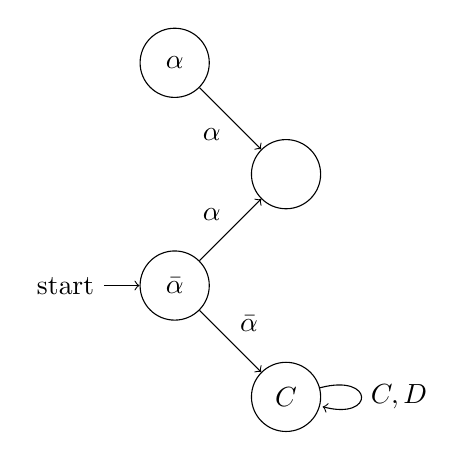
\begin{tikzpicture}[node distance=2cm]
          \node[state, initial] (c_0) {$\bar{\alpha}$};
          \node[state] (c_1) [below right of=c_0] {$C$};
          \node[state] (c_prime) [above right of=c_0] {};
          \node[state] (c) [above left of=c_prime] {$\alpha$};

          \path[->] (c_0) edge node [above right] {$\bar{\alpha}$} (c_1);
          \path[->] (c_1) edge [loop right] node [right] {$C,D$} ();
          \path[->] (c_0) edge node [above left] {$\alpha$} (c_prime);
          \path[->] (c) edge node [below left] {$\alpha$} (c_prime);
        \end{tikzpicture}
        \caption{Constructon of invasion strategy, used in the proof of \cref{evolutionarystable1}}
        \label{invasionstrategy}
      \end{figure}


      \begin{claim}
        Given the above construction of $s_2$, the following inequalities hold:
      \begin{align*}
        v_{s_1}(s_1) &\leq (1-p)^2 \gamma + 2(1-p)p R + p^2  R \\ 
        v_{s_1}(s_2) &\leq (1-p) \gamma + p T \\
        v_{s_2}(s_1) &\geq (1 - p) \gamma  + p S \\
        v_{s_2}(s_2) &\geq (1-p)^{2} R + 2 (1-p) p (\tfrac{S + T}{2}) + p^2 \gamma .
      \end{align*}
      \end{claim}

      Before proving this claim, we will use it to finish our proof of \cref{evolutionarystable1}.

      Now, we simply compute $F(s_2) - F(s_1)$, which we want to show is greater than 0.
      \begin{align*}
        F(s_2) - F(s_1) &= \\
        &= (1 - \epsilon) \cdot v_{s_2}(s_1) + \epsilon \cdot v_{s_2}(s_2) - (1 - \epsilon) \cdot v_{s_1}(s_1) - \epsilon \cdot v_{s_1}(s_2) \\
        &= (1 - \epsilon) (\gamma + p(\ldots)) + \epsilon (R + p(\ldots)) - (1-\epsilon) (\gamma + p(\ldots)) - \epsilon (\gamma + p(\ldots)) \\
        &= \epsilon (R - \gamma) + p(\ldots)
      \end{align*}

      We know that $R - \gamma > 0$ by our initial assumption. Clearly, since $(\ldots)$ is some polynomial in $p$, given an $\epsilon$ we can find a sufficiently small $p$ such that the full expression is positive. This proves that $s_2$ can invade $s_1$, and thus, that $s_1$ is not $\epsilon$-invadable for this value of $p$. In conclusion, then $s_1$ is not evolutionarily stable, which concludes the proof of \cref{evolutionarystable1}.

    \end{proof}

    \begin{proof}[Proof of \cref{claimpayoffs}]
      We can prove this using either of the two definitions.
    \end{proof}

    \subsection{Evolutionarily Stable Strategies Exist}

    Unfortunately, we have no proof of \cref{pavlovtheorem}.

    We note that the $2R > T + P$ condition is necessary. Otherwise, the AllD strategy would be able to invade Pavlov. We see this by noting that $\lim_{p \to 0} v_{s_2}(s_1) = T + P$ if $s_2$ is AllD and $s_1$ is Pavlov, and that AllD is better against itself than Pavlov is against it.



    \section{Discussion of Model}
    \label{sectiondiscussion}



    \subsection{Other Potential Models}

    Right now we have only modeled noise in perception. One could think of another possible kind of noise: a ``failure of the mind,'' which perhaps could be modeled instead by a probability $p$ of being transported to any random state, instead. This would create ergodicity which is nice.

    \iffalse

    \section{Appendix: Time average distributions}

    We might have periodicity, but for our purposes, we might as well extend the definition and look at periodic distributions as stationary too. The following two lemmas help with that.

    \begin{lemma}
      Given a starting distribution $v$ and a Markov matrix $M$, for every $\epsilon > 0$, there will exist a $k$ such that $|vP^{nk} - vP^{mk}| < \epsilon$ for all $n$ and $m$ $> 0$.
    \end{lemma}

    This proves that a Markov chain will always reach a periodic state.

    \begin{lemma}
      Suppose distributions form a chain $p_1 \to p_2 \to \cdots \to p_n \to p_1$. Then $\pi = \frac{p_1 + \ldots p_n}{n}$ is stationary.
    \end{lemma}

    This proves that we're able to talk about stationary distributions even when they don't really actually exist.

    \fi

    \section{Appendix: Probablistic Automata}

    OHHHHHHH. THIS WILL HELP WITH MY PROOF????? THIS IS EXACTLY WHAT I'M TRYING TO DO IN MY PROOF RIGHT????? YEAHHHH, NO.

    In this paper, we have considered strategies that make a deterministic move based on what they perceive. One could also imagine strategies that attaches a certain probability distribution to a perceived input, and chooses their next action based on that. In this appendix we show that these can be reduced to the deterministic ones, and thus that all results for the deterministic ones also hold for the probabilistic ones.

    Proof idea: we can use cycles in the Markov chain with n total outputs, x of which are to state 1, to model getting to state 1 with probability x / n. this assumes that the outputs are of low enough probability, which can be achieved by chaining together lots of (1-p) transitions, which go to 0.

    the hard part of this is showing that modifying the finite automaton like this won't hurt us. in fact, it would certainly not hurt us if not every state had to give an output. but that doesn't work for our model i think. so there are certainly things to think about here.



    \bibliography{bibliography.bib}
    \bibliographystyle{acm}


\end{document}